\documentclass[output=paper]{langscibook} 
\author{Yranahan Traoré\lastand Caroline Féry \affiliation{University of Frankfurt}}
% % \abstract{This article examines the syllable structure in Fòʔò, a dialect of Tagbana spoken in Côte d’Ivoire. The underlying syllable structure is limited to C(C)V and V syllable, thus syllables with an onset and syllables consisting with a nucleus and nothing else. The onset can be complex, although it is limited to two positions which are restricted in their order by the sonority sequence principle. By contrast, the surface syllables are the result of phonological changes that take place in specific morphological environments. Vowel deletion happens regularly when two identical vowels are separated by a consonant in the context C$_1$V$_1$.C$_2$V$_2$. there is also a process of liquid deletion that simplifies underlying complex onsets. However, when the complex onset is the result of vowel deletion, liquid deletion does not apply: The two processes—syllable become more complex or syllable are simplified—are in a counterfeeding relation to each other. The last process that is described is fusion of two monosyllabic morphemes into a single syllable. If the second morpheme is wí with a glide in its onset, the fusion results in a CV syllable with a round vowel. Otherwise the emerging syllable is CVC where the first CV is the entire first morpheme and the second C is the consonant of the second morpheme. The results of the study of syllable structure is tested on loanwords, where syllables’ repairs take place. For instance, codas are avoided by epenthesis and unallowed initial vowels trigger epenthesis of an onset segment [h]. It is also shown how the constraints on syllable structure repair loanwords in Fròʔò}
\abstract{This article examines the syllable structure in Fròʔò, a dialect of Tagbana spoken in Côte d’Ivoire. In our analysis, the underlying syllable structure in Fròʔò is limited to C(C)V and V. Other surface syllable shapes, such as CVC, are the result of synchronic morphophonological processes. These processes include the formation of surface complex onsets through vowel deletion, the simplification of underlying complex onsets through liquid deletion, and the merger of bisyllabic CVCV sequences into monosyllables (CVC and CV). Evidence of these phonological process can also be found in loanwords, where syllable repairs take place.}
\title{Syllable structure and loanword adaptation in Fròʔò}

\begin{document}
\maketitle

\section{Introduction}
\label{sec:traore:introduction:1}

This article studies the syllable structure in Fròʔò (Tagbana), a Senoufo (Gur) language of Côte d’Ivoire (see \citealt{Clamens1952}, \citealt{Manessy1962}, \citealt{Herault1973}, \citealt{Miehe2012}, \citealt{MieheEtAl2012}) and the effects that syllabic restrictions have on loanword adaptation. \sectref{sec:traore:syllable_structure:2} introduces the underlying syllable structure and the basic phonotactic rules of Fròʔò. \sectref{sec:traore:resyllabification:3} discusses three resyllabification processes. First, two kinds of vowel deletion are introduced: one leading to coda emergence, and another one leading to complex onsets.  The second resyllabification process is liquid deletion leading to onset simplification. \sectref{sec:traore:merging_process:4} examines the process of merging two monosyllabic morphemes into a single syllable. \sectref{sec:traore:loanwords:5} focuses on the way phonotactic restrictions influence loanword adaptations. \sectref{sec:traore:conclusion:6} summarises and concludes.

Before turning to syllable structure, let us briefly introduce the phonemic inventory of Fròʔò, its lexical and grammatical tones and the nominal class system. The consonants are shown in \tabref{tab:traore:consonants:1}. 
There are 22 consonants, 10 of which are stops and two are voiceless fricatives, but there is no voiced fricative. The 10 stops are divided into voiceless and voiced ones with five places of articulation: labial, alveolar, palatal, velar and labio-velar. Two laryngeal obstruents are present as well: [ʔ] and [h]. Additionally, there are six sonorants, four of which are nasals. The remaining sonorants are two glides, [j] and [w], and two liquids, [l] and [r]. The Fròʔò consonant system is close to that of other ​​Gur languages, although some differences emerge as well. For instance, voiced fricatives have been shown to exist in other Gur languages.

\begin{table}
\begin{tabularx}{\textwidth}{XXssssss}
\lsptoprule
 &  & labial & alveolar & palatal & velar & labio-velar & glottal\\\midrule
\multirow{2}{*}{Plosive} & voiceless & p & t & c & k & kp & ʔ\\
& voiced & b & d & ɟ & g & gb & \\
Fricative &  & f & s &  &  &  & h\\
Nasal &  & m & n & ɲ & ŋ &  & \\
Glide &  &  &  & j &  & w & \\
Lateral &  &  & l &  &  &  & \\
Rhotic &  &  & r &  &  &  & \\
\lspbottomrule
\end{tabularx}
\caption{Fròʔò consonants \label{tab:traore:consonants:1}}
\end{table}

Fròʔò has seven oral vowels that can be long in some environments, in particular before a heteromorphemic [r] or [l]. All vowels have nasal correspondents, except for the mid [+ATR] ones, [e] and [o], that are never nasalized; thus all in all the language shows 12 vowels, as shown in Figures~\ref{fig:traore:short_vowels:1} and~\ref{fig:traore:nasal_vowels:2}. In this article, IPA is used (Fròʔò has no written system).

\begin{figure}[b]\RawFloats
\begin{minipage}{.5\textwidth}\centering
\begin{vowel}
    \putcvowel{i}{1}
    \putcvowel{e}{2}
    \putcvowel{ɛ}{3}
    \putcvowel{a}{15}
    \putcvowel{u}{8}
    \putcvowel{o}{7}
    \putcvowel{ɔ}{6}
\end{vowel}
\caption{Short vowels \label{fig:traore:short_vowels:1}}
\end{minipage}\begin{minipage}{.5\textwidth}\centering
\begin{vowel}
    \putcvowel{ĩ}{1}
    \putcvowel{ɛ̃}{3}
    \putcvowel{ã}{15}
    \putcvowel{ũ}{8}
    \putcvowel{ɔ̃}{6}
\end{vowel}
\caption{Nasal vowels \label{fig:traore:nasal_vowels:2}}
\end{minipage}
\end{figure}\clearpage

Fròʔò has three level tones, high (H), mid (M) and low (L). There are no contour tones. The syllable is the tone bearing unit (TBU) and every syllable in every word carries its own tone, regardless of the category and the length of the word. In other words, all vowels in the language bear one of these three tones. Some examples of (near-) minimal pairs appear in \REF{ex:traore:tonal_change_aspect_change:1}.\footnote{Every noun belongs to a nominal class, see below. In the examples in \tabref{tab:traore:minimal_pairs:3}, the numbers “7” and “1” indicate that the nouns belong to class 7 or class 1. The word \textit{kɔ́-lɔ́ } `monkey' consists of a lexical root and a class marker of class 1.}

\begin{table}
\caption{Tonal minimal pairs\label{tab:traore:minimal_pairs:3}}
\begin{tabular}{lll}
 \lsptoprule
 \multicolumn{1}{c}{H} & \multicolumn{1}{c}{M} & \multicolumn{1}{c}{L} \\\midrule
hũ̀-mũ̀7  ‘oil’ & hũ̄-mũ̄7 ‘worship’ & hṹ-mṹ7  ‘the drink’\\
 pà̰1 ‘monitor lizard & pā̰     ‘to come’ &  \\
 fà̰1 ‘bamboo tree &   fā̰      ‘to build’& \\
  &  ɉīō5  `house’ & ɉíó  ‘to carry’\\
  & kɔ̄lɔ̄   ‘to cough’ &  kɔ́-lɔ́ ‘monkey-\textsc{cm1}’\\
  fìὲːrὲ6  ‘the sham’ & pέːrέ  ‘to sell’ \\\lspbottomrule
\end{tabular}
\end{table}

Tones play a large role in the grammatical domain, as exemplified in \REF{ex:traore:tonal_change_aspect_change:1}, where a change in grammatical tone signifies a change in tense/aspect/mood of the utterance. 

\begin{exe}
    \ex Tonal changes due to aspect changes \label{ex:traore:tonal_change_aspect_change:1}
    \begin{xlist}
     \ex \gll kí              {mã̀ }           glã́ \\
         \textsc{pro}.\textsc{obj}     \textsc{pro}{}-2\textsc{sg}    please\\
         \trans `It will please you'
    \ex \gll  kí               mã́             glã́ \\
            \textsc{pro}.\textsc{obj}     \textsc{pro}{}-2\textsc{sg}   like\\
            \trans `Did it please you?'
    \ex \gll kī              mã̄              glã̀ \\
        \textsc{pro}.\textsc{obj}    \textsc{pro}{}-2\textsc{sg}   like\\
        \trans  `Make it please you!'
    \end{xlist}

\end{exe}

Combinations of tones in the nominal domain reveal the existence of floating tones in part of the vocabulary, compare \REF{ex:traore:floating_tones:2a} with \REF{ex:traore:floating_tones:2b}. The high tone on the verb \textit{síɔ́} in \REF{ex:traore:floating_tones:2b} is the result of a floating tone on the noun (marked with a superscript H) that spreads up to the verb.\footnote{\textsuperscript{} Thanks to Annie Rialland for working this out with us.}  

\begin{exe}
 \ex Floating tones \label{ex:traore:floating_tones:2}
\begin{xlist}
 \ex   \gll àtò:lò            +    sīɔ̄                  →          àtò:lò sīɔ̄  \label{ex:traore:floating_tones:2a}\\
          spoon-\textsc{cm}2    {}       {to buy}   {}            {}\\
        \trans `to buy a spoon’
 \ex  \gll àblòʔò\textsuperscript{H}      +    sīɔ̄                  →          àblòʔò síɔ́ \label{ex:traore:floating_tones:2b}\\
      peanut-\textsc{cm}5           {}    {to buy}          {}          {}\\
      \trans ‘to buy a peanut’
\end{xlist}
\end{exe}
 

 Nouns are the result of a sequence of a lexical root and an overt or a covert class marker (CM). \tabref{tab:traore:nominal_classes:4} provides an overview of the nominal classes in Fròʔò (see Traoré and Féry, unpublished, for nouns and nominal classes). Every noun belongs to one of seven nominal classes, which are classified according to the phonological form of their class marker and/or associated functional morphemes, i.e., the morphemes in an agreement relation with the head noun (see \citealt{Corbett1991}). Six of the classes form gender pairs of singular and plural, but the nouns in class 7 are mass nouns or nouns denoting properties. This class has no corresponding plural. When the CM is covert, we do not indicate it as a CM in the gloss. The lexical root is written with its class instead, e.g., \textit{pà̰1 ̰} ‘monitor lizard’ and \textit{wótìɔ̀1} ‘python’.

\begin{table}
\caption{Overview of the nominal classes of Fròʔò and their class markers \label{tab:traore:nominal_classes:4}}
\begin{tabularx}{\textwidth}{Xss}
\lsptoprule
Class markers (CM) & \multicolumn{2}{c}{Examples of nouns of each class}\\
\midrule
\textbf{Class} \textbf{1} (sg. of gender 1)         & hō-lō                     &  wótìɔ̀1   \\
several CM, including Ø                             & elephant-\textsc{cm1}     &  python\\
\tablevspace
\textbf{Class} \textbf{2} (pl. of gender 1)         & hō-bēlē                   & wótìɔ̀-hélé\\
CM: [-hele], [-bele], -lV                           & elephants-\textsc{cm2}    & pythons{}-\textsc{cm2}\\
\tablevspace
\textbf{Class} \textbf{3} (sg. of gender 2)         & lāː-lā                    & kpē-lē\\
CM: [-lV]                                           & belly{}-\textsc{cm3}      & knife{}-\textsc{cm3}\\  
\tablevspace
\textbf{Class} \textbf{4} (pl. of gender 2)         & lā-ʔālā                   & kpē-gēlē\\
CM: [-ʔVlV, -gele]                                  & bellies-\textsc{cm4}      & knives{}-\textsc{cm4}\\
\tablevspace
\textbf{Class} \textbf{5} (sg. of gender 3)         & jē-gē                     & āfɔ̃̄-ŋɔ̃̀ \\
CM: [-gV]/[-ŋV]/[-ʔV] or Ø                          & month-\textsc{cm5}        & new thing\-{}-\textsc{cm5}\\
\tablevspace
\textbf{Class} \textbf{6} (pl. of gender 3)         & jēː-rē                    &  āfɔ̃̄:-rɔ̃̀\\
CM: [-rV]                                           & months-\textsc{cm6}       & new things{}-\textsc{cm6}\\
\tablevspace
\textbf{Class} \textbf{7} (sg. of gender 4)         & ɲũ̄-mũ &    wɛ̄-bɛ̄ \\ 
CM: [-mV]                                           & water-\textsc{cm7}        & foliage{}-\textsc{cm7}\\
\lspbottomrule
\end{tabularx}
\end{table}

\section{Underlying syllable structure and phonotactics}
\label{sec:traore:syllable_structure:2}

Two underling syllable structures are present in Fròʔò: the first type of syllable consists only of a nucleus (V or [n]), and the second type consists of an onset + nucleus, see \REF{ex:Traore:UnderlyingSyllableStructure:4}. In the latter case, the onset can be simple or complex, consisting of maximally two consonants, thus (C)CV.

\begin{exe}
    \ex \label{ex:Traore:UnderlyingSyllableStructure:4}Fròʔò underlying syllable structures 
    
    \begin{forest}
        [ σ  [V] ]
        \end{forest}
    \hspace{1cm}
    \begin{forest}
         [ σ  [n] ]
        \end{forest}
    \hspace{1cm}
    \begin{forest}
        [ σ  [C(C)] [V]]
        \end{forest}
\end{exe}

\subsection{V syllable: Nucleus only}
\label{sec:v_syllable:2a}

As far as syllables consisting of only a nucleus are concerned, only [a] can start a word as illustrated in \REF{ex:traore:WordInitiala:5}, see \citet{Herault1973} for the same observation for Tákpɛ̃́r, another dialect of Tagbana; [a] can be oral or nasal.\footnote{The only exception is the interjection \textit{è.hé} ‘yes, ok’.} 

\begin{exe}\setlength\multicolsep{0pt}
    \ex \label{ex:traore:WordInitiala:5}[a]/[ã] in word-initial position
    \begin{multicols}{2}\raggedcolumns
     \begin{xlist}
         \ex \gll ā.jlē-ʔè\\
                mirror-\textsc{cm5} \\
              \trans `mirror'\\
        \ex \gll ā.wrē-ʔē\\
            {something itchy-\textsc{cm5}}\\
            \trans `something itchy'
        \columnbreak
        \ex à.plè3 \\
            `shade'
        \ex ã̀.gù1 \\
            `traditional dance'
        \ex \gll ã̄.gō-lò \\
                mount-\textsc{cm3}\\
            \trans `mount'
     \end{xlist}
     \end{multicols}
 \end{exe}
 
Word-medially, all vowels can be a nucleus, see two examples in \REF{ex:traore:VowelHiatusPosition:6}, each of which contains a CM consisting only of a vowel.\largerpage[2]

 \begin{exe}\setlength\multicolsep{0pt}
     \ex \label{ex:traore:VowelHiatusPosition:6}Vowel at hiatus position
     \begin{multicols}{2}\raggedcolumns
     \begin{xlist}
         \ex \gll pì-ɔ̀ \\
            child-\textsc{cm1}\\
        \trans `child'
        \columnbreak\ex \gll kā.fū-ō \\
             sweat-\textsc{cm5}\\
             \trans `sweat'
     \end{xlist}
     \end{multicols}
 \end{exe}
        

Word-initially, before all vowels other than [a], [h] or another consonant is needed; see \REF{ex:traore:hInitialWords:7} for words starting with [h].  In loanwords starting with a vowel, [h] is inserted word-initially, see \sectref{sec:traore:loanwords:5}.

 \begin{exe}\setlength\multicolsep{0pt}
     \ex {[h]} initial words \label{ex:traore:hInitialWords:7}
     \begin{multicols}{2}\raggedcolumns
     \begin{xlist}
         \ex hēːrē\\
            `to press'
        \ex  hɔ̄ʔɔ̄  \\
            `to cook'
        \ex hòʔó \\
            `to stoop'
        \columnbreak
        \ex  hɛ̰́   \\
            `where'
        \ex \gll hí-ʔí\\
            feather-\textsc{cm5}\\
            \trans `feather'
        \ex  \gll hú-ʔú \\
            thorn-\textsc{cm5}\\
            \trans `thorn'
     \end{xlist}
     \end{multicols}
 \end{exe}

Syllables consisting of a nasal only are the subject of \sectref{sec:traore:syllabicnasals:2d}

\subsection{ CV syllable: onset + nucleus}
\label{sec:traore:cvsyllable:2b}

All consonants can occupy the word-initial onset position except for the glottal stop [ʔ] and [r], both of which do not occur in this position. In \REF{ex:traore:initialConsonants:8}, monosyllabic words are used for illustration.

\begin{exe}
    \ex \label{ex:traore:initialConsonants:8}
    \begin{multicols}{3}\raggedcolumns
        \begin{xlist}
            \ex pũ̄1\\
                `dog'
            \ex bā7\\
                `this'
            \ex tō1\\
                `father'
            \ex díː\\
                `so, that'
            \ex cã́ \\
                `to fall'
            \ex ɉɛ̀ \\
                `to wake up'
            \ex kā\\
                `to break'
            \columnbreak\ex gũ̄1 \\
                `tortoise'
            \ex  kpē\\
                `to take'
            \ex gbò1 \\
                `gnat'
            \ex  fã̄ \\
                `to build'
            \ex  sɛ̄ \\
                `produce'
            \ex hɛ̃́ \\
                `where'
            \ex mĩ̀\\
                `I, me'
            \columnbreak\ex nũ̀1 \\
                `ox'
            \ex ɲĩ\\
                `to fill'
            \ex ŋã̄ \\
                `this one'
            \ex  jō\\
                `to say'
            \ex  wī  \\
                `him'
        \end{xlist}
    \end{multicols}
\end{exe}

Vowel lengthening is triggered by a following liquid, [r] or [l], as shown in \REF{ex:traore:vowelLengtheningExamples:9}. Liquids at the beginning of word final syllables often are the initial consonant of a class marker, but not always. The examples in \REF{ex:traore:vowelLengtheningExamples:9} have a heteromorphemic liquid, except for \REF{ex:traore:vowelLengtheningExamples:9f}, in which the last syllable is part of the lexical root. 
 
 \begin{exe}
     \ex \label{ex:traore:vowelLengtheningExamples:9}
     \begin{multicols}{2}
        \begin{xlist}
            \ex \gll lōː-rō\\
            mango-\textsc{cm}6\\
            \trans `mangoes'
            \ex \gll kāː-lā\\
            problem-\textsc{cm}3'\\
            \trans `problem'
            \ex \gll pĩ̀ː-rĩ̀   \\
            tam-tam-\textsc{cm}6\\
            \trans `tam-tams'
            \columnbreak
            \ex \gll pũ̄ː-lũ̄ \\
            dog-\textsc{cm}2\\
            \trans `dogs'
            \ex \gll pìː-lì\\
            child-\textsc{cm}2\\
            \trans `children'
            \ex  ɉàː.rà1   \label{ex:traore:vowelLengtheningExamples:9f}\\
            `lion'
        \end{xlist}
     \end{multicols}
 \end{exe}
 
Not all vowels lengthen before a liquid, as shown in \REF{ex:traore:lackOfVowelLengthening:10}. This happens when the vowel follows [ʔ]. In this case, it is deleted or pronounced as a short and weak vowel (see \sectref{sec:traore:vowel_deletion_ccv:3b}
 for vowel deletion). Thus, the sequence [ʔVrV] blocks lengthening of the vowel following [r]. 

 \begin{exe}\setlength{\multicolsep}{0pt}
    \ex \label{ex:traore:lackOfVowelLengthening:10}
    \begin{multicols}{2}
        \begin{xlist}
            \ex fīʔī.rí\\
            `to frighten'
            \ex  híʔí.rí\\
            `to shiver'
            \columnbreak
            \ex ɲɔ̃́ʔɔ̃́.rɔ̃́\\
            `to move'
            \ex hùʔù.rú\\
            `to spin'
        \end{xlist}
    \end{multicols}
 \end{exe}

\subsection{ CCV syllables: complex onset + nucleus}
\label{sec:ccvsyllable:2c}

Consonant clusters in the onset are quite common in Fròʔò. They are mostly regulated by the sonority sequencing principle, which states that the sonority of segments rises toward the nucleus of a syllable and lowers away from it (see for example \citealt{Clements1990} for this principle). Stops are the least sonorous segments and low vowels the most sonorous ones, as illustrated in \REF{ex:traore:sonorityHierarchy:11}.

\begin{exe}
    \ex Sonority hierarchy \label{ex:traore:sonorityHierarchy:11}\\
    Stops\hspace{.3cm}Fricatives\hspace{.3cm}Nasals\hspace{.3cm}Liquids\hspace{.3cm}Glides\hspace{.3cm}High vowels\hspace{.3cm}Low vowels\\
    \begin{tikzpicture}[node distance=2cm]
    \node (A) at (0,0) {};
    \node (B) at (11,0) {};
    \draw [->] (A) -- (B);
    \end{tikzpicture}
\end{exe}

In Fròʔò, the maximum number of consonants in the onset is two. Nearly all consonants, except for [s], [h], [r] and the glottal stop [ʔ], can be followed by [l] and [r]; even the glides [w] and [j] can form complex onsets with a liquid, in violation of the sonority principle, since glides are more sonorous than liquids. There is a restriction against a sequence of two coronals if the second one is the lateral, thus [tl], [dl], [nl] and [rl] do not occur as complex initial onsets.

\tabref{tab:traore:complexOnsets:4} lists all possible word-initial complex onsets. 

 
\begin{table}
    \caption{Complex onsets\label{tab:traore:complexOnsets:4}}
\resizebox{\textwidth}{!}{\begin{tabular}{*{21}{c}}
% % \lsptoprule %% Table was transposed
% % {} & m           & l           & r \\\midrule
% % p  & \textminus  & +           & +\\
% % b  & \textminus  & +           & +\\
% % t  & \textminus  & \textminus  & +\\
% % d  & \textminus  & \textminus  & +\\
% % c  & \textminus  & +           & +\\
% % ɟ  & \textminus  & +           & +\\
% % k  & +           & +           & +\\
% % g  & +           & +           & +\\
% % kp & \textminus  & +           & +\\
% % gb & \textminus  & +           & +\\
% % f  & \textminus  & +           & +\\
% % s  & \textminus  & \textminus  & +\\
% % h  & \textminus  & +           & \textminus \\
% % ʔ  & \textminus  & \textminus  & +\\
% % m  & \textminus  & +           & +\\
% % n  & \textminus  & \textminus  & +\\
% % ɲ  & \textminus  & +           & +\\
% % ŋ  & \textminus  & +           & +\\
% % w  & \textminus  & +           & +\\
% % j  & \textminus  & +           & +\\
% % \lspbottomrule
\lsptoprule
   & p  &  b  & t  & d  & c  & ɟ  & k  & g  & kp & gb & f  & s  & h  & ʔ  & m  & n  & ɲ  & ŋ  & w  & j \\\midrule
m  & \textminus  & \textminus  & \textminus  & \textminus  & \textminus  & \textminus  & +  & +  & \textminus  & \textminus  & \textminus  & \textminus  & \textminus  & \textminus  & \textminus  & \textminus  & \textminus  & \textminus  & \textminus  & \textminus  \\
l  & + & + & \textminus  & \textminus  & + & + & + & + & + & + & + & \textminus  & + & \textminus  & + & \textminus  & + & + & + & + \\
r  &  + &  + &  + &  + &  + &  + &  + &  + &  + &  + &  + &  + &  \textminus &  + &  + &  + &  + &  + &  + &  +\\
\lspbottomrule
\end{tabular}}
\end{table}

\noindent Words initial complex onsets are illustrated in \REF{ex:traore:complexOnsetWordInitial:12}. 

 \begin{exe}
    \ex Complex word-initial onsets \label{ex:traore:complexOnsetWordInitial:12}
    \nopagebreak
    \begin{multicols}{2}
    \begin{xlisti}
        \ex \glll [pl]: \textbf{pl}ɔ̀.ʔɔ̀ \\
            {}      bamboo-\textsc{cm}5\\
            {} ‘bamboo’\\ 
        \ex \gll [pr]: \textbf{pr}ò6\\
            {}  `chip'\\
        \ex \gll [bl]:        \textbf{bl}ɔ̄ \\
            {}      `plowed'\\
        \ex \gll [br]:      \textbf{br}é.ʔé \\
            {} {`to boil'}\\
        \ex \gll [tr]:        \textbf{tr}á.ʔá\\
            {}      {`to stick up'}\\
        \ex \glll [dr]:      \textbf{dr}è.ʔè \\
            {}      shift-\textsc{cm}5\\
            {}      `shirt'\\
        \ex \glll [cl]:       \textbf{cl}ɛ̄.mũ̀ \\
            {} woman-\textsc{cm}7\\
            {} `womanhood'\\
        \ex \gll [cr]:        \textbf{cr}ɛ̄.ʔɛ̄  \\
            {}          {`to expand'}\\
        \ex \gll [ɉl]:         ɉ\textbf{l}ì.ʔí\\
            {}          `wise'\\
        \ex  \gll [ɉr]:        ɉ\textbf{r}ɛ̀.ʔɛ́ \\
            {}          {`to fly'}\\
        \ex \glll [kl]:       \textbf{kl}ã\={}.ʔã\`{}~\\
            {} seat-\textsc{cm}5\\
            {} `seat'\\
        \ex \glll  [kr]:       \textbf{kr}ɔ.ʔɔ \\
            {} car-\textsc{cm}5\\
           {}  `car'\\
        \ex \gll [km]:      \textbf{km}ɔ́\\
            {}      {`to beat'}\\
        \ex \gll [gm]:      \textbf{gm}ɔ́\\
            {}      `beaten'\\
        \ex \glll [gl]:       \textbf{gl}ē.ʔè\\
            {}          tamis-\textsc{cm}5\\
            {} ‘tamise’\\
        \ex \gll [gr]:       \textbf{gr}ā̰  \\
            {}      `dirty'\\
        \ex  \glll [kpl]:      \textbf{kpl}ɛ̀.ʔɛ̀ \\
            {}          former-\textsc{cm}5\\
            {}          `former'\\
        \ex \glll [kpr]:     \textbf{kpr}ā.ʔā\\
            {}          {sugar cane-\textsc{cm}5}\\
            {} {`sugar cane'}\\
        \ex \gll [gbl]:     \textbf{gbl}ɛ̀ːr\\
            {}          `beginning'\\
        \ex \gll [gbr]:     \textbf{gbr}è.ʔè\\
            {}          `unripe'\\
        \ex \glll [fl]: \textbf{fl}ĩ̀.ʔĩ̀  \\
            {} furuncle-\textsc{cm}5\\
            {} `furuncle'\\
        \ex \gll [fr]:        \textbf{fr}ɔ̄.ʔɔ̄ \\
            {} {`to scrub'}\\
        \ex \glll [sr]:        \textbf{sr}ɛ́.ʔɛ́\\
            {}      prayer-\textsc{cm}5\\
            {}      `prayer'\\
        \ex \glll [hl]:   \textbf{hl}ã̄-ʔã̄\\
            {} leg-\textsc{cm}5\\
            {} `leg'\\
        \ex \glll [hr]:      \textbf{hr}ō6\\
                {}          meal\\
                {}          `meals'\\
        \ex \glll [ml]:      \textbf{ml}ã̄-ʔã̄ \\
            {}          fight-\textsc{cm}5\\
            {}          `fight'\\
        \ex \glll  [mr]:       \textbf{mr}ũ̀.ʔũ̀ \\
            {}  corosol-\textsc{cm}5\\
            {}  `corosol'\\
        \ex \glll [nr]:      \textbf{nr}ɛ̃̀\\
            {}          root-\textsc{cm}6\\
            {}          `roots'\\
        \ex \gll [ɲl] \textbf{ɲl}ɔ̃́.ʔɔ̃́\\
            {}  {`to write'}\\
        \ex \gll [ɲr]:      \textbf{ɲr}ã́.ʔã́ \\
            {}      {`to hook'}\\
        \ex \glll [ŋl]:       \textbf{ŋl}ɔ̃́-ʔɔ̃́\\
            {} dream-\textsc{cm}5\\
            {} `dream'\\
        \ex \gll [ŋr]:       \textbf{ŋr}ɔ̃̄.ʔɔ̃̄    \\
            {}  {`to push'}\\
        \ex  \gll [wl]:       \textbf{wl}ɛ̀-ʔɛ̀ \\
                {}          day-\textsc{cm}5\\
        \ex \gll [wr]:       \textbf{wr}ē.ʔē  \\
                {}          `short'\\
        \ex \glll [jl]:         \textbf{jl}ɛ̄.mɛ̄ \\
            {}      clean-\textsc{cm}7\\
            {} `cleanliness'\\
        \ex \glll [jr]:       \textbf{jr}ā.ʔā\\
            {}              thing-\textsc{cm}5\\
            {}              `thing'\\
        \end{xlisti}
    \end{multicols}
\end{exe}


Only [k] and [g] can form an initial complex onset with [m], but the segment clusters [km] and [gm] are only attested in a few words. \citet{Herault1973} analyze them as the nasal counterparts of [kp] and [gb] when the following vowel is nasal, see examples in \REF{ex:traore:velarPlusNasalComplexOnset:13}. In other words, in their analysis [km] and [gm] are allophones of underlying /kp/ and /gb/. An alternative explanation is that the vowel following [km] and [gm] is subject to nasal harmony. That explains why the following vowel is always nasal. In fact, [kp] and [gb] can be followed by a nasal vowel, and this distributional fact speaks against the allophonic nature of [km] and [gm], see the examples in \REF{ex:traore:velarPlusNasalComplexOnset:13}. Word-medial complex onsets are listed in \REF{ex:traore:wordMedialComplexOnsets:15}.


\begin{exe}\setlength{\multicolsep}{0pt}
    \ex \label{ex:traore:velarPlusNasalComplexOnset:13}
    \begin{multicols}{2}
    \begin{xlist}
        \ex \textbf{km}ɔ̃́ \\
            `to hit'
        \ex \textbf{km}ã̄-ʔã̄  \\
            `nice'\\
        \ex \gll \textbf{km}ɔ̃́.ʔɔ̃́-lɔ̃̄ \\
            fireplace-\textsc{cm}3\\
            \trans `fireplace'\\
        \ex \gll lā.\textbf{gm}ã̄.mũ̄  \\
            belly-kind-\textsc{cm}7\\
            \trans `kindness'\\
    \end{xlist}
    \end{multicols}
\end{exe} 

 \begin{exe}\setlength{\multicolsep}{0pt}
    \ex \label{ex:traore:14}
     \begin{multicols}{2}
        \begin{xlist}
            \ex \gll kpɛ̃̄-mũ̀   \\
                daylight-\textsc{cm}7\\
                \trans `daylight'\\
            \ex \gll kpã̀dàː-là\\
               {funeral yard-\textsc{cm}3}\\
              \trans `funeral yard'\\
             \ex \gll lāgbã̄-mũ̄ \\
                anger-\textsc{cm7}\\
                \trans `anger'\\
        \end{xlist}
     \end{multicols}
 \end{exe}
 
 \begin{exe}\setlength{\multicolsep}{0pt}
     \ex Word-medial complex onsets \label{ex:traore:wordMedialComplexOnsets:15}
    \begin{multicols}{2}
     \begin{xlisti}
        \ex \glll [pl]:    tī.\textbf{pl}ɔ̄-ʔɔ̄ \\
            {}  ground-\textsc{cm}5\\
            {} `ground'\\
        \ex \glll [pr]:     tì.\textbf{pr}ì-ʔì\\
            {}  fresh-\textsc{cm}5\\
            {} `freshness'\\
        \ex \glll [bl]:    à.\textbf{bl}ò-ʔò\\
            {}      peanut-\textsc{cm}5\\
            {} `peanut'\\
        \ex  \glll [br]:    à.\textbf{br}à.ʔà\\
            {}  {`to bargain'}\\
            {}  {}\\
        \ex \glll [tr]:    kpà.\textbf{tr}ō-ʔō\\
            {}   whip-\textsc{cm}5\\
            {}  `whip'\\
        \ex \glll [dr]: kā.fĩ̄.n.\textbf{dr}ī-ʔī\\
            {}  {umbilical cord-\textsc{cm}5}\\
            {}  {`umbilical cord'}\\
        \ex \glll  [cl]:   kā.\textbf{clē}{}-ʔē \\
            {}  bone-\textsc{cm}5\\
            {} `bone'\\
        \ex \glll [ɉl]:     n.ɉ\textbf{l}é.ʔè\\
            {}   wall-\textsc{cm}5\\
            {}  `wall'\\
        \ex  \glll [ɉr]:      kɔ.ɉ\textbf{r}ɛ́.lɛ́ \\
            {}  mangoose-\textsc{cm}3\\
            {}  `mangoose'\\
        \ex \glll [kl]:    tì.\textbf{kl}ɔ̰̀.ʔɔ̰̀\\
            {}  `long'\\
            {}  {}\\
        \ex  \glll [kr]:     kā.\textbf{kr}ā.ʔ\\
            {}  junk-\textsc{cm5}\\
            {}  `junk'\\
        \ex \glll [km]: a.\textbf{km}ɔ̃̄ː-rɔ̃̀\\
            {}  strike-\textsc{cm6} \\
            {}  {`the strikes'}\\
        \ex \glll [gm]:    la.\textbf{gm}ã̄-m(ũ̀)  \\
            {} belly-kind-\textsc{cm}7\\
            {}   `kindness'\\
        \ex \glll [gl]:   hã̄.\textbf{gl}ā.ʔà \\
            {} bow-\textsc{cm}5 \\
            {} `bow'\\
        \ex \glll [gr]:    bà.\textbf{gr}à-ʔà\\
            {}  hoe-\textsc{cm5} \\
            {}  `hoe'\\
        \ex \glll [gbl]:  kã́.\textbf{gbl}ò-ʔò\\
            {} cudgel-\textsc{cm}5 \\
            {} ‘cudgel’\\
        \ex \glll [gbr]    ā.\textbf{gbr}ē.ʔē\\
            {}   unripe-\textsc{cm5}\\
            {}  `unripe'\\
        \ex \glll [fl]:    tū.\textbf{fl}ɛ̄-ʔɛ̄ \\
            {}  wind-\textsc{cm}5\\
            {}  `wind'\\
        \ex \glll [fr]:      kā.\textbf{fr}ɛ.ʔɛ\\
            {}  {`to apologize'}\\
            {}  {}\\
        \ex \glll [ml]:  nã̀.\textbf{mã̄.ʔã̀ ~}\\
            {} {`name of person'}\\
            {} {}\\
        \ex \glll [mr]:     ká\textbf{mr}ɔ̃̀-ʔɔ̃̀ \\
            {}   agouti-\textsc{cm}5\\
            {}   `agouti'\\
        \ex \glll [ŋl]:    mṹ.\textbf{ŋã̀-ʔã̀ }\\
            {}  ember-\textsc{cm}5\\
            {} `ember' \\
        \ex \glll [jl]:      a.\textbf{jl}ē-ʔē \\
            {}   mirror-\textsc{cm}5  \\
            {} `mirror'\\
        \ex \glll [ɲr]:   ā.\textbf{ɲr}ɔ̃̄-ŋɔ̃̄ \\
            {}  en-\textsc{cm}5 \\
            {} `pen'\\
        \ex \glll  [hr]:    kā.\textbf{hr}ē-ʔè\\
            {}  cashew-apple-\textsc{cm}5\\
            {}  `cashew-apple'\\
        \ex \glll [wl]:  kū.\textbf{wl}ɛ̀.ʔɛ̀ \\
            {} {`before yesterday'}\\
            {} {}\\
        \ex \glll  [wr]:    ā.\textbf{wr}ē-ʔē\\
            {} {something itchy-\textsc{cm}5}\\
            {} {`something itchy'}\\
     \end{xlisti}
     \end{multicols}
 \end{exe}

\subsection{ Syllabic nasals}
\label{sec:traore:syllabicnasals:2d}

As mentioned above, Fròʔò has tautosyllabic complex onsets involving the nasals [n], [m], [ɲ] and [ŋ], which can be followed by liquids, except for [nl] which has been shown above to be excluded on other grounds. These clusters obey the sonority sequencing principle. Some additional examples appear in \REF{ex:traore:nasalWithLiquids:16}.

 \begin{exe}\setlength{\multicolsep}{0pt}
    \ex Nasal-liquid onsets \label{ex:traore:nasalWithLiquids:16}
     \begin{multicols}{3}
        \begin{xlist}
            \ex \glll [ml]:       \textbf{ml}ã̄-ʔã̄ \\
                {}  war-\textsc{cm}5 \\
                {} `war'\\
            \ex \glll [mr]:       \textbf{mr}ũ̀-ʔũ̀ \\
                {}   corosol-\textsc{cm}5\\
                {}  `corosol'\\
            \ex \gll [nr]:      \textbf{nr}ɛ̃̀6 \\
                {}  `root'\\
        \end{xlist}
     \end{multicols}
 \end{exe}


In other cases, a nasal consonant precedes a less sonorous segment. In this case, the nasal makes a syllable on its own: syllables in Fròʔò may consist of a nasal consonant and nothing else. There is no prenasalized obstruent in Fròʔò. These syllables only appear in word-initial position. These nasals are followed by a stop (or an affricate) in the next syllable’s onset, see \REF{ex:traore:wordInitialSyllabicNasalConsonants:17} for examples.  


 \begin{exe}\setlength{\multicolsep}{0pt}
     \ex Word-initial syllabic nasal consonants \label{ex:traore:wordInitialSyllabicNasalConsonants:17}
     \begin{multicols}{3}
     \raggedcolumns
     \begin{xlist}
        \ex ǹ.klō\\ 
            `name of person'\\
        \ex ǹ.dā(hā)\\
            `name of person'\\
        \columnbreak
        \ex ń.cɛ\\
            `name of person'\\
        \ex  \gll \={n}.ɉlē-ʔē\\
            wall-\textsc{cm}5\\
            \trans `wall'\\
        \columnbreak
        \ex  \gll \'{ŋ}.glɛ̰́3\\
            pestle\\
            \trans `pestle'\\
        \ex   \`{m}.bìɔ\\
            `ship'\\
     \end{xlist}
     \end{multicols}
 \end{exe}

The structure of a nasal syllable followed by another syllable is shown in \REF{ex:traore:syllabicNasalTree:18}. It is also relevant when the second syllable has a complex onset, like in \textit{n.klō} ‘name of person’.

 \begin{exe}
     \ex Syllabic nasal \label{ex:traore:syllabicNasalTree:18}\\
         \begin{forest}
        [ word  [σ [n]] [σ [c][ɛ̄ ]]]]
        \end{forest}
 \end{exe}

When the stop following the nasal is voiced, the initial syllabic nasal assimilates to the articulator of the following stop. Before bilabial [b], the nasal is labial [m]; before [d] and [ɉ], it is coronal [n]; and before the voiced dorsal [g] and labio-dorsal [gb], it is dorsal [ŋ]. \tabref{tab:traore:syllabicNasalVoicedStop:5} shows the possible combinations between nasals and voiced stops word initially. 

\begin{table}
    \centering
\begin{tabularx}{.7\textwidth}{XXXXXX} 
\lsptoprule
& b & d & ɉ & g & gb\\\midrule
m & + & \textminus  & \textminus  & \textminus  & \textminus \\
n & \textminus  & + & + & \textminus  & \textminus \\
ŋ & \textminus  & \textminus  & \textminus  & + & +\\
\lspbottomrule
\end{tabularx}
    \caption{Syllabic nasal + voiced stop \label{tab:traore:syllabicNasalVoicedStop:5}}
    \label{tab:my_label}
\end{table}

The feature filling process in \figref{ex:traore:consonantClusterFeatureFillingProcess:19} assumes that the nasal consonant [N] is underlyingly unspecified for its place of articulation and that it acquires an articulator from the following stop. However, it could also be the case that the articulator of the nasal is specified as [coronal] and that it loses its coronality as a result of spreading of the articulator node.

    \begin{figure}
        \centering
    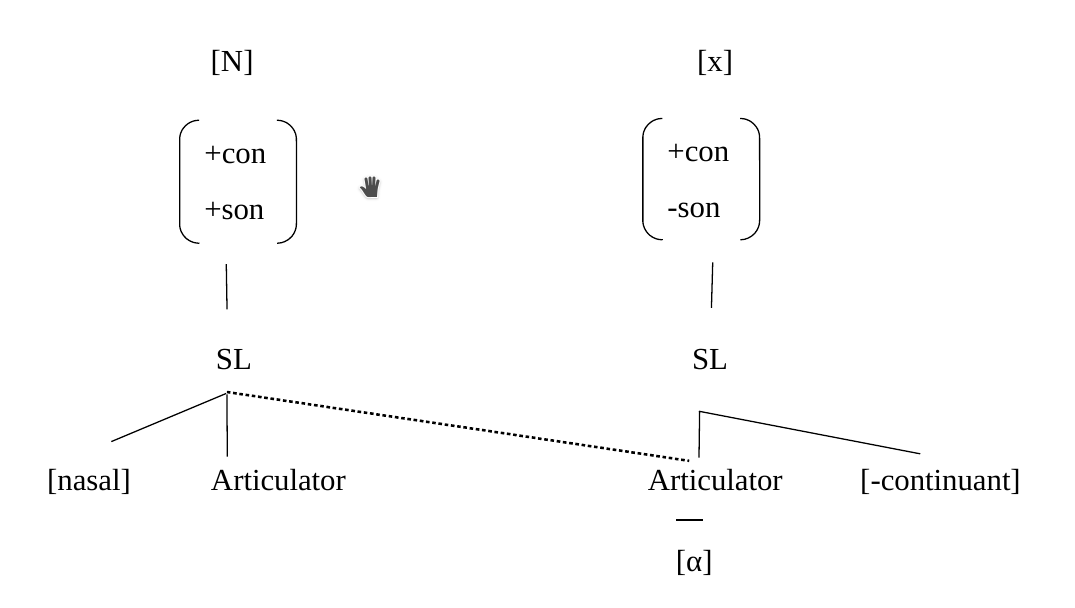
\includegraphics[width=8.2cm]{figures/featureAssignmentProcess.png} % width calculated from image resolution at 300dpi
        \caption{Consonant cluster with a nasal, where [x] stands for any plosive segment \label{ex:traore:consonantClusterFeatureFillingProcess:19}}
    \end{figure}

\section{Resyllabification}
\label{sec:traore:resyllabification:3}

In some cases, the underlying syllable structures that were described in \sectref{sec:traore:syllable_structure:2} are subject to modification. This section deals with the following resyllabification processes: vowel deletion of the second vowel in a sequence of two vowels in two adjacent syllables, leading to CVC syllables (\sectref{sec:traore:vowel_deletion_to_cvc:3a}); vowel deletion of the first vowel in two adjacent syllables leading to CCV syllables (\sectref{sec:traore:vowel_deletion_ccv:3b}); and liquid deletion, a process of onset simplification (\sectref{sec:traore:liquid_deletion:3c}).\footnote{Vowel deletion and liquid deletion have also been documented for Syer, another Gur language, see \citet{Dombrowsky2015}.} Furthermore, Fròʔò also has a morphophonological process: two monosyllabic function words are fused into a single syllable, see \sectref{sec:traore:merging_process:4}. 

\subsection{ Vowel deletion leading to CVC syllables}
\label{sec:traore:vowel_deletion_to_cvc:3a}

If some conditions are met, when two morphemes come together, the last vowel of the first morpheme or word deletes, and a coda is created. We refrain from calling the process ``vowel syncope'', since that would imply that it is an unstressed vowel that is deleted. However, there is no evidence whatever for stress in Fròʔò. Vowel deletion in Fròʔò touches all vowels equally.\footnote{High vowels are not deleted more easily than mid or low vowels, as is the case in the neighboring Bamana, Colloquial Bambara (see \citealt{Green2014}).}

\begin{exe}
\ex Coda creation through vowel deletion \label{ex:traore:codaCreationVowelDeletion:20}\\
    CV.CV → CVC
 \end{exe}

The result of vowel deletion appears in the third column of the examples in \REF{ex:traore:vowelDeletionSecondSyllable:21}, showing a sequence of two nouns, or of a noun (or a verb) and an article or a class morpheme. 

 \begin{exe}
    \ex Vowel deletion in the second syllable \label{ex:traore:vowelDeletionSecondSyllable:21}\\
    \begin{tabularx}{.8\textwidth}{l l l l l}
        tī.cēː.rē   &   +   &   fɔ́.lɔ́                  &   →       & tī.\textbf{cēːr}{}-fɔ́-lɔ́  \\
        `madness'   &   {}  &   `owner-\textsc{cm1}'    &   {}      & {`mad person-\textsc{cm}1'}\\
                    &       &                           &           &                           \\
        tī-ʔī       &   +   &  kà                       &   →       &  \textbf{tīʔ}{}-kà \\
        `tree-\textsc{cm}5' & {} & \textsc{ind.art}.    &   {}      &  {`a tree'}\\
                            &       &                           &           &               \\
        fɛ́ː.rɛ́       &    + &     mũ̀                    &   →       & \textbf{fɛ́ːr}-mũ̄ \\
        {`happy person'} & {} & \textsc{cm}7            &   {}      & `happiness-\textsc{cm}7'\\
                                             &       &                           &           &               \\
       tã́.ʔã́  &  +  & lV                        &  →        & \textbf{tã́ʔ}-lã̄  \\
        `to walk'       &   & \textsc{cm}3              &           & `walk-\textsc{cm3}'\\
                                             &       &                           &           &               \\
        klò.ʔó       &   +  & lV                        &  →        & \textbf{klòʔ}{}-ló\\
        ‘to roll’   &       &  \textsc{cm}3             &           & `fact of rolling-\textsc{cm}3'\\
                                             &       &                           &           &               \\
        pɛ́:.rɛ́    &  +    & lV                        &   →       & \textbf{pɛ́:r}{}-lɛ́   \\
        `to sell'   &       & \textsc{cm}3              &           &  `sale-\textsc{cm3}'\\
    \end{tabularx}
 \end{exe}

In \REF{ex:traore:tripleVowelDeletion:21}, the vowel deletion process takes place three times.      

 \begin{exe}
    \ex \gll kà-ʔà             +     fɔ́.lɔ́                  + krɔ̀ʔɔ̀            +   ka                  →      \textbf{kàʔ-fɔ́l-krɔ̀ʔ}-kà \label{ex:traore:tripleVowelDeletion:21}\\
            `village-\textsc{cm}5'  {} `chief-\textsc{cm1}' {} `car-\textsc{cm}5'   {}  \textsc{ind.art}.   {}       {‘chief of village’s car’}\\
 \end{exe}
          
The application of vowel deletion and subsequent coda creation are subject to three restrictions. First, the deleted vowel is identical to the preceding one. This happens when a CM is added to a lexical root, in which case it is the result of vowel harmony. The CMs are of the form CV with a specified C, dependent on the class of the noun, and an unspecified V, which is a total copy of the last vowel of the root. 

In case the final vowel is prespecified and is thus not the result of vowel harmony, the final vowel cannot delete. %
%(22) doesn’t show the failure of sentence internal position délétion, so I would first say … the final vowel cannot delete, see (22). Indeed, even in sentence internal position they cannot delete (with adding an example if you want).
The words in \REF{ex:traore:lexicalRootsWithoutCM:22} are lexical roots that do not take an overt CM. Moreover, the second vowel is not identical to the first one.%\largerpage
 
\noindent\parbox{\textwidth}{\begin{exe}\setlength{\multicolsep}{0pt}
    \ex\label{ex:traore:lexicalRootsWithoutCM:22}
    \begin{multicols}{4}\raggedcolumns
    \begin{xlist} 
    \ex  jù.gò5
      \trans  `head'
    \ex dã̀..gò1
       \trans `sheet'
    \ex nũ̀..bú.ó1
    \trans `friend'
    \ex wó.tì.ɔ̀1
      \trans `python'
  \end{xlist}\end{multicols}
 \end{exe}}

The second restriction is that only consonants that start a CM can become the coda of a syllable. As a result, the sonorants [m, l, r, ŋ], the voiced stops [b] and [g], and the glottal stop can appear in a coda after vowel deletion. All other consonants cannot.\footnote{\citet{Green2014} show that in Bamana, syncope results in high sonority codas, but low sonority ones are excluded. This is not always the case in Fròʔò, although high sonority codas are more frequent.}

Third, vowel deletion is blocked at the end of a sentence, see the examples in \REF{ex:traore:vowelDeletionBlockedAtEndOfSentence:24}. In both cases, the last vowel would delete in the sentence-internal position, but fails to do so in sentence-final position. The words ending in a consonant in these examples have lost their final vowel, which is always a copy of the preceding vowel.

\begin{exe}
    \ex \label{ex:traore:vowelDeletionBlockedAtEndOfSentence:24}
    \begin{xlist}
   \ex \gll kàɉíó:-rdā  wō  lá  dɛʔ pé  nã́  tí  hóʔ\textbf{ó}\\ 
            camps-\textsc{cm}6     \textsc{rel.pro}    \textsc{pro.1pl}    \textsc{asp} show    \textsc{pro.3pl}     to    \textsc{pro.3pl}     burn\\
         \glt    ‘The camps that we showed to them have burned’ 
    \ex \gll tī-ʔ   gā  kí  tō  nã̀dò-ʔ  nã̄  kí  nĩ́  kpã̀  gbã̄ -ŋ\textbf{ã̄ }\\
              tree-\textsc{cm}5 \textsc{rel.pro}    \textsc{pro.3sg}    {fall down}  yam-\textsc{cm}5  on    \textsc{pro.3sg}   \textsc{aux}    big-\textsc{cm}5\\
              \glt `The tree that has fallen down on yam is big.'
\end{xlist}
\end{exe}

\subsection{ Vowel deletion leading to CCV syllables}
\label{sec:traore:vowel_deletion_ccv:3b}

In \REF{ex:traore:vowelDeletionFirstSyllable:25}, vowel deletion applies in the first syllable of a lexical root. In such a case, the deleted vowel is not that of a CM, but that of the root. However, it is again identical to the following vowel. The first example (\ref{ex:traore:vowelDeletionFirstSyllable:25}a) shows a lexical root plus a class marker playing the role of a nominalizer suffix. The second example (\ref{ex:traore:vowelDeletionFirstSyllable:25}b) shows a derived noun plus an additional class marker playing the role of a derivational suffix. It is conspicuous that this second vowel deletion concerns lexical root vowels. In Fròʔò, as in other West African languages, some vowels may be called ``weak'' and are subject to deletion in the right context (see \citealt{Sande2017} for similar effects in Guébié, a Kru language). Weak vowels contrast with ``strong'' vowels that never delete.\pagebreak

    \begin{exe}
        \ex Vowel deletion in the first syllable\label{ex:traore:vowelDeletionFirstSyllable:25}\\
        \begin{tabularx}{.5\textwidth}{l l l l l}
        wé.lé           &        +    & ʔV                  &       →       &        \textbf{wlé}{}-ʔé \\
        `to look'       &    {}       &   \textsc{cm}5      &      {}       &       `look-\textsc{cm}5'\\
                        &           &                       &               &       `the look'          \\
                                &           &                       &               &     \\
        cɛ̄-lɛ̄          &     +      & mũ̀              &       →       &    \textbf{clɛ̄}-mũ̀  \\
        `woman-\textsc{cm}1'    &   &   \textsc{cm}7        &               &   `woman-\textsc{cm}7'\\
                                &           &                       &               &  `womanhood'   \\
        \end{tabularx}
    \end{exe}

\subsection{ Liquid deletion}
\label{sec:traore:liquid_deletion:3c}

Another resyllabification process in Fròʔò involves liquid deletion in the second position of a complex onset. The syllable structure is simplified as shown in \REF{ex:traore:liquidDeletion:26}: only the less sonorous first consonant C is preserved.

\begin{exe}
    \ex Liquid deletion \label{ex:traore:liquidDeletion:26}\\
    ClV / CrV → CV
\end{exe}

Liquid deletion takes place in the first morpheme in a sequence of two adjacent morphemes, the examples in \REF{ex:traore:liquidDeletionLexicalRootsCM:27} show lexical roots plus CM. In this case, liquid deletion is restricted to identical vowels separated by a CM starting with [r], as illustrated.
    
    \begin{exe} 
        \ex Vowel deletion in lexical roots plus \textsc{cm} \label{ex:traore:liquidDeletionLexicalRootsCM:27}\\
        \begin{tabularx}{.8\textwidth}{l l l l l l}
            a. & drɛ̃̀        &   +   &   \textsc{cm}6    &   →   & \textbf{dɛ̃̀ː}{}-    rɛ̃̀ \\               
             &  bee           &       &                   &       &  `bees'\\
                            &       &                   & &      &       \\
          b. & kàbrɛ̀             &   +   &  \textsc{cm}6     &   →   & kà\textbf{bɛ̀ː}{}-rɛ̀\\
          & grasshopper       &       &                   &       & `grasshoppers'\\
                                      &       &           &        &       &       \\
            c. & krà             &  +    &   \textsc{cm}6    &   →   &   \textbf{kàː}{}-rà\\
        &     file            &       &                   &       &   `files'\\
        \end{tabularx}
    \end{exe}

Another context in which liquid deletion applies is a sequence of a noun and an adjective, see \REF{ex:traore:liquidDeletionCompounds:28}. These words are compounds consisting in two lexical roots, a nominal one and an adjectival one. The class marker is not always there, but if it is required, it is located at the end of the compound. Note that in (\ref{ex:traore:liquidDeletionCompounds:28}a) neither \textit{plɔ̀} nor \textit{plè} requires a CM in isolation, and the resulting compound has no CM. The same holds for other compounds in \REF{ex:traore:liquidDeletionCompounds:28}. The vowels do not need to be identical. The first consonant of the adjectives is sometimes voiced. It is not clear what triggers voicing.

 \begin{exe}
     \ex Liquid deletion in compounds \label{ex:traore:liquidDeletionCompounds:28}\\
     \begin{tabularx}{.8\textwidth}{l l l l l l }
       a. & plɔ̀      &      +    &  plè  &  →    &    \textbf{pɔ̀ }-blè \\
        & bamboo  &       {}  & small & {}    & `small bamboo'\\
        &        &           &       &       &               \\
        b. & krɔ̀      &       +   &  plè  &  →    &  \textbf{kɔ̀ }-plè\\
        & car     &       {}  &   small   &   &   `small car'\\
        &         &           &       &       &               \\
        c. & hlã̄     &   +       &  klɔ̃̄  &  →    & hã̄ -glɔ̃̄ \\
        & leg     & {}        & long      & {}    & `long leg'\\
        &        &           &       &       &               \\
        d. & kámrɔ̃̀ &  +    & kpɔ̄       &  →    &  ká\textbf{mɔ̃̀}{}-gbɔ̀-ʔɔ̀\\
        & agouti      &       & big       &       &   `big agouti-\textsc{cm}5'\\
        &         &           &       &       &               \\
        e. & kāhrē   &   +      &    kēːrè   &   →   & kā\textbf{hē}{}-gērè \\
        & cashew  &           &  field    &       & `field of cashew'\\
        &        &           &       &       &               \\
       f. & klō      &   +       &   kpɔ̄     &   →  & \textbf{kō}{}-gbɔ̄-ʔɔ̄  \\ 
        & road    &           & big       &       & `big road-\textsc{cm}5'\\
         &       &           &       &       &               \\
        g. & kā.clē  &   +       &   kpɔ̄      &   →  & kā.\textbf{cē}{}-gbɔ̄-ʔɔ̄  \\
        & bone    &           &   big     &       & `big bone-\textsc{cm}5'\\
     \end{tabularx}
 \end{exe}

Liquid deletion also takes place if the compound is preceded by yet another lexical root, see examples in \REF{ex:traore:compundPrecededByLexicalRoot:29}.

\begin{exe}
    \ex Liquid deletion in nominal compounds\label{ex:traore:compundPrecededByLexicalRoot:29}\\
    \begin{tabularx}{.8\textwidth}{l l l l l l}
    a. & pìɔ   &     +    &  \textbf{pɔ}{}-blè   &   →   &  pìɔ.\textbf{p}ɔ.blé\\
    & child   &       & small bamboo          &       & `child’s small bamboo'\\
                    &           &       &       &               \\
    b. & tō    &     +  & \textbf{k}ɔ̃.plè\-  &   →       & tō.\textbf{k}ɔ.plè \\
        & father  &       & small car         &           & `father’s small car' \\
    \end{tabularx}
\end{exe}

Liquid deletion in monosyllabic nouns without a CM is not possible. The words in \REF{ex:traore:NoLiquidDeletionMonosyllabicNouns} illustrate that in such a case, the liquid is not deleted.        
    \pagebreak
    \begin{exe}
        \ex No liquid deletion in monosyllabic nouns \label{ex:traore:NoLiquidDeletionMonosyllabicNouns}\\
        \begin{tabularx}{.7\textwidth}{l l l l l l }
        a. & klò1     &       +   &   plè    &   →  &        klò-plè (*kò-plè  )\\
        & country   &         &  small    &       &   `small country'\\
         &           &       &           &       &                   \\
        b. & klɛ̃̄3    &  +    &  plè     &   →  &    klɛ̃̄-plé\\   
        & post        &       &   small   &       & `small post'\\        
        &            &       &           &       &                   \\
        c. & krò5      &     +   &   plè     &   →   & krò-plè       \\             
        & rubber    &         & small     &       & `small rubber'\\  
        &            &       &           &       &                   \\
        d. & plò     &    +      & plè       &   →  &    plò-plè-ʔélé\footnote{The last noun (\ref{ex:traore:NoLiquidDeletionMonosyllabicNouns}d) \textit{plò} does not have a singular equivalent.}\\
        & plants   &          & small     &       & `small plants-\textsc{cm}4'\\ 
        \end{tabularx}
    \end{exe}
    
Liquid deletion takes place in words with a non-high vowel. A liquid preceded by a high vowel, [i] or [u], as in \REF{ex:traore:31}, cannot be deleted. 

\begin{exe}\setlength{\multicolsep}{0pt}
    \ex  No liquid deletion before a high vowel  \label{ex:traore:31}\\
    \begin{multicols}{3}\raggedcolumns
    \begin{xlist}
        \ex  \glll frù-ʔù         frùː-rù\\
              mat-\textsc{cm}5    mat-\textsc{cm}6\\
              `mat' `mats'\\
        \columnbreak\ex \glll klù-ʔù          klùː-rù\\
        way-\textsc{cm}5      way-\textsc{cm}6\\
        `way' `ways'\\
        \columnbreak\ex \glll   flĩ̀-ʔĩ̀   {flĩ̀ ː-rĩ̀ }\\
        spot-\textsc{cm}5      spot-\textsc{cm}6\\
        `spot' `spots'\\
    \end{xlist}\end{multicols}\end{exe}

Liquid deletion does not happen in verbs.
In all examples, liquid deletion takes place in the first element of a compound. The second compound does not lose its liquid.

\begin{exe}
  \ex No liquid deletion in the second element of compounds\label{ex:traore:32}\\
  \begin{xlist}
    \ex \gll pìɔ̀      +          plɔ̀                           →            pìɔ̀.\textbf{pl}ɔ̀-ʔɔ̀    *(pìɔ̀.\textbf{p}ɔ̀-ʔɔ̀)\\
    child               {}    bamboo                           {}         {}  {}\\
    \trans ‘child’s bamboo’  
    \ex  \gll tō            +          krɔ                           →            tō.\textbf{kr}ɔ̀-ʔɔ̀  \\            father         {}       car                            {}            {}\\
    \trans ‘father’s car’
    \end{xlist}
 \end{exe}

\section{Merging process in Fròʔò}\label{sec:traore:merging_process:4}

Merging (or portmanteau building) denotes the process of making one word out of two. In Fròʔò, two independent monosyllabic function morphemes are merged into a single syllable, for instance two pronouns, or an auxiliary and a pronoun. The pronouns may have different functions in the sentence: subject and one or two objects for instance. There are two ways of achieving merging in Fròʔò, the first of which is fusion, resulting in a CV syllable, and the second of which is resyllabification with vowel deletion and consequent coda creation (CVC), of the same type described in \sectref{sec:traore:vowel_deletion_to_cvc:3a}

\subsection{Merging as fusion}
\label{sec:traore:merging_as_fusion:4a}

In the fusion process, only one syllable is formed out of two: the onset of the first word is preserved and the resulting vowel has features from all remaining segments. First examples appear in \REF{ex:traore:33}. In these fused morphemes, two monosyllabic pronouns on the left are pronounced in one syllable, as shown to the right of the arrows. In all cases, the onset of the first pronoun is kept: these are, respectively, [k], [t], [l], [m], [w] and [p]. The fused segment is always [u] and is the result of fusing [i] from the first pronoun and [wí] from the second pronoun. In all examples, all words have a high tone, and unsurprisingly the fused morpheme also has a high tone.
    
   
    \begin{exe}
    \ex Fusion of two pronouns \label{ex:traore:33}\\
    \begin{xlist} 
        \ex \gll kí              wí                ɲã̀                   →            \textbf{kú}      ɲã̀ \\  
              \textsc{pro1.3sg}     \textsc{pro3.3sg}      see           {}         {}          {}\\
              \trans `it has seen him'\\
         \ex \gll  tí               wí                ɲã̀                 →            \textbf{tú}    ɲã̀  \\ 
          \textsc{pro1.3pl}    \textsc{pro3.3sg}      see                   {}          {} {}\\
          \trans `they have seen him'\\
        \ex \gll  lí                wí                ɲã̀                  →            \textbf{lú}    ɲã̀ \\
              \textsc{pro2.3sg}    \textsc{pro3.3sg}      see                {}         {}          {}\\
             \trans `it has seen him'\\
         \ex \gll  mĩ́               wí                ɲã̀                     →            \textbf{m}ṹɲã̀ \\
               \textsc{pro.1sg}        \textsc{pro3.3sg}      see                 {}            {}          {}\\
               \trans `I have seen him'\\
        \ex \gll wí              wí                ɲã̀                 →            \textbf{wú}ɲã̀\\
            \textsc{pro3.3sg}     \textsc{pro3.3sg}      see          {}        {}      {}\\
            \trans `he has seen him'\\
        \ex \gll pí              wí                ɲã̀                 →            \textbf{pú}    ɲã̀\\
        \textsc{pro4.3sg}    \textsc{pro3.3sg}      see              {}             {}          {}\\
        \trans `they have seen him'\\
        \end{xlist}
 \end{exe}

The features involved in the fusion process are illustrated in \REF{ex:traore:34} and \REF{ex:traore:35}. The features of the resulting vowel are a compromise between the features of the original vowels and [w], the initial consonant of the second pronoun. Since both vowels are [+high], this feature is kept. The feature [labial] of [w] is translated into vocalic [round] and [round] in Fròʔò only appears on back vowels. For this reason, [i] becomes [u] in the fused version.

\begin{exe}
    \ex\label{ex:traore:34}
        \begin{tikzpicture}[baseline=(ki.base),node distance=2cm]
            \node [anchor=base] (ki) at (0,2) {ki};
            \node [anchor=base] (wi) at (2,2) {wi};
            \node [anchor=base] (ku) at (1,0) {ku};
            \draw [->] (ki) -- (ku);
            \draw [->] (wi) -- (ku);
        \end{tikzpicture}
 \end{exe}

\begin{exe}
    \ex Features of the fused segments [i], [w] and [i] \label{ex:traore:35}\\
    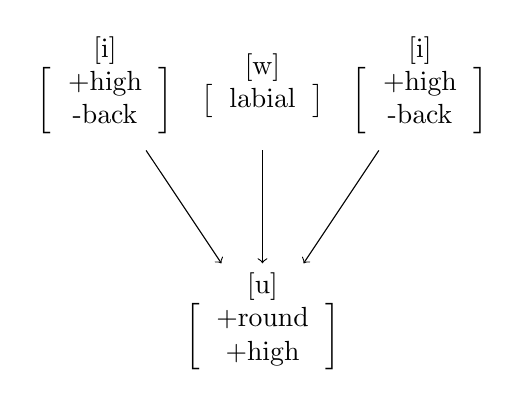
\begin{tikzpicture}[baseline=(i.base),node distance=3cm]
    \node[align=center,anchor=base] (i) at (0,3) {{[i]}\\$
\left[
  \begin{tabular}{c}
  +high\\
  -back
  \end{tabular}
\right] 
$\\};
    \node[align=center,anchor=base] (w) at (2,3) {{[w]}\\$
\left[
  \begin{tabular}{c}
 labial
  \end{tabular}
\right] 
$\\};
    \node[align=center,anchor=base] (i2) at (4,3) {{[i]}\\$
\left[
  \begin{tabular}{c}
  +high\\
  -back
  \end{tabular}
\right] 
$\\};
\node[align=center,anchor=base] (u) at (2,0) {{[u]}\\$
\left[
  \begin{tabular}{c}
  +round\\
  +high
  \end{tabular}
\right] 
$\\};
    \draw [->] (i) -- (u);
    \draw [->] (w) -- (u);
    \draw [->] (i2) -- (u);
    \end{tikzpicture}
\end{exe}


However, the fused vowel is not always [u]. In \REF{ex:traore:36}, it is [ɔ], the result of fusing [ã] and [i]. Notice that [o] cannot be nasalized and [ɔ̃] is used instead.

\begin{exe}
     \ex \gll mã\'{}            wí                   ɲã̀                →        mɔ̃́    ɲ    ã̀ \label{ex:traore:36}\\
               \textsc{pro.2sg}     \textsc{pro3.3sg}        see            {}       {}      {}\\
              \trans `you have seen him'\\
 \end{exe}

In this case, a compromise is needed between [low] from [ã] and [+high] from [i]. The result is the mid back vowel [ɔ̃], a round nasal segment by default. Nasality of the first word is preserved, and height is a compromise. As before [round] is derived from the labiality of the glide [w]. 

\begin{exe}
  \ex Features of the fused segments [a], [w] and [i]\\
  \begin{tikzpicture}[baseline=(a.base),node distance=2cm]
        \node[align=center,anchor=base] (a) at (0,3) {{[a]}\\$
\left[
  \begin{tabular}{c}
  low\\
  nasal
  \end{tabular}
\right] 
$\\};
        \node[align=center,anchor=base] (w) at (2,3) { {[w]}\\$
\left[
  \begin{tabular}{c}
  labial
  \end{tabular}
\right] 
$\\};
    \node[align=center,anchor=base] (i) at (4,3) {{[i]}\\$
\left[
  \begin{tabular}{c}
  +high\\
  -back
  \end{tabular}
\right] 
$\\};
    \node[align=center,anchor=base] (ɔ) at (2,0) { {[ɔ̰̄]}\\$
\left[
  \begin{tabular}{c}
  round\\
  -high\\
  nasal
  \end{tabular}
\right] 
$\\};
    \draw [->] (a) -- (ɔ);
    \draw [->] (w) -- (ɔ);
    \draw [->] (i) -- (ɔ);
    \end{tikzpicture}
 \end{exe}
 
Further examples of fused morphemes appear in \REF{ex:traore:38}. 

\begin{exe}
    \ex \label{ex:traore:38}
        \begin{xlist}
            \ex \gll pé               wí               ɲã̀                 →          \textbf{pó}   ɲã̀\\  
                  \textsc{pro3.3pl}     \textsc{pro3.3sg}    see             {}             {}      {}\\
                  \trans `they have seen him'\\
             \ex \gll ké              wí              ɲã̀                 →          \textbf{kó}    ɲã̀\\
                   \textsc{pro3.3sg}     \textsc{pro3.3sg}    see       {}          {}          {}\\
                \trans `they have seen him'\\
    \end{xlist}
 \end{exe}

In \REF{ex:traore:39}, two monosyllabic pronouns \textit{pé} ‘they’ and \textit{wí} ‘him, her’ are fused. The fusion segments are [é] from the first pronoun and [wí] the second pronoun and the result of the fusion is [ó], again a back vowel in order to keep the feature [labial] from [w].  

\begin{exe}
\ex Features of the fused segments [é], [w] and [í]\label{ex:traore:39}\\
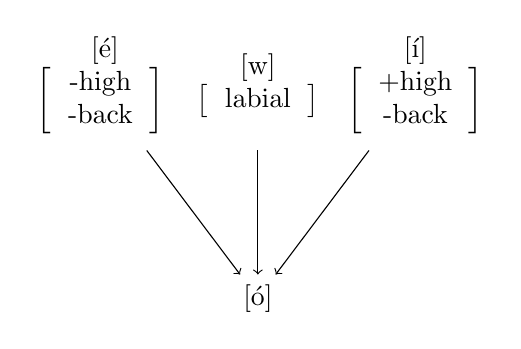
\begin{tikzpicture}[baseline=(e.base),node distance=2cm]
 \node[align=center,anchor=base] (e) at (0,2) {{ [é] }\\$
\left[
  \begin{tabular}{c}
  -high\\
  -back
  \end{tabular}
\right] 
$\\};
    \node[align=center,anchor=base] (w) at (2,2) {{[w]}\\$
\left[
  \begin{tabular}{c}
  labial
  \end{tabular}
\right] 
$\\};
    \node[align=center,anchor=base] (i) at (4,2) {{[í]}\\$
\left[
  \begin{tabular}{c}
  +high\\
  -back
  \end{tabular}
\right] 
$\\};
    \node (o) at (2,0) {[ó]};
    \draw [->] (e) -- (o);
    \draw [->] (w) -- (o);
    \draw [->] (i) -- (o);
\end{tikzpicture}
\end{exe}
 

\subsection{Merging as resyllabification with vowel deletion}
\label{sec:traore:merging_as_resyll_with_vowel_deletion:4b}
Fusion of the kind illustrated in \sectref{sec:traore:merging_as_fusion:4a} is not always a possible outcome. In the following examples, it is still the case that two monosyllabic function words are fused into one, and the result is thus a portmanteau word in each case, but the process is different: the onset of the second morpheme becomes the coda of the syllable made by the first morpheme. The examples in \REF{ex:traore:40} show how the lateral [l] of the object pronoun \textit{lí} becomes the coda of the syllable of the first pronoun. A similar process of vowel deletion was already illustrated in \sectref{sec:traore:vowel_deletion_to_cvc:3a} An important difference is now that the deleted vowel does not need to be identical to the preceding one, see \REF{ex:traore:40f}.

    \begin{exe}
        \ex Fusion of two pronouns leading to a syllable with coda:   CV + CV → CVC \label{ex:traore:40}
        \begin{xlist}
            \ex \gll kī              lí                  ɲã̀                →        kíl ɲã̀ \label{ex:traore:40a}\\ 
             \textsc{pro1.3sg}     \textsc{pro3.3sg}      see             {}          {}\\
             \glt `it has seen hit'
            \ex \gll tī               lí                  ɲã̀               →        tíl ɲã̀ \label{ex:traore:40b}\\ 
            \textsc{pro1.3pl}     \textsc{pro3.3sg}      see                 {}         {}\\
            \glt `they have seen hit'
            \ex \gll  lī                lí                  ɲã̀                →        líl  ɲã̀ \label{ex:traore:40c} \\
                \textsc{pro2.3sg}     \textsc{pro3.3sg}      see                {}  {}\\
                \glt `it has seen hit'
            \ex \gll wī              lí                  ɲã̀                →        wíl ɲã̀ \label{ex:traore:40d}\\
                \textsc{pro3.3sg}     \textsc{pro3.3sg}      see             {}         {}\\
                \glt `he has seen him'
            \ex \gll kē              lí                  ɲã̀                →        kél ɲã̀ \label{ex:traore:40e}\\
                \textsc{pro2.3pl}       \textsc{pro3.3sg}    see        {}      {}\\
                \glt `they have seen him'
            \ex \gll pē              lí                  ɲã̀                →        pél ɲã̀ \label{ex:traore:40f}\\
                \textsc{pro3.3pl}     \textsc{pro3.3sg}      see         {}     {}\\
                \glt `they have seen him'
        \end{xlist}
    \end{exe}

\section{Loanwords}
\label{sec:traore:loanwords:5}

 Loanwords are a good place to verify the generalizations obtained for constraining the syllable structure of a language. They validate syllable structural processes in Fròʔò that have been discussed in the previous sections of this article.

Loanword phonologies have received much attention in the last decades, see for instance \citet{Ito1995},  \citet{Peperkamp2003} and others. They shape the phonological structure of new words entering the language and impose native phonotactic and segmental constraints on them. Speakers of a language confronted with the task of articulating foreign words adjust the phonological shape of these words to render them more native. This implies that the segments of foreign words need to be adapted to the native phonemic inventory in case they are not there from the start. Moreover, and this is what we are primarily interested in here, the constraints on the syllable structure of the borrowing language needs to be respected. \citet{Silverman1992} made a distinction between two adaptation tasks: at the ``perceptual level'', the acoustic input, or the acoustic image that the speaker has of the foreign word, is interpreted as a string of native segments. At the ``operative level'', all segments are assigned licit positions in the syllables. However, the two levels are not always clearly separated from each other. An illicit consonant in the coda for instance can be accommodated in (at least) two ways: either it is replaced by a licit consonant that may happen to be similar to the original one. An illicit consonant in the coda for instance can be accommodated. For example, it could be replaced by a licit consonant that may happen
to be similar to the original one, the syllable structure could be repaired by adding a vowel so that the illicit coda is adapted as the onset of a
new syllable, or the coda could be deleted altogether. Consider first the examples in \REF{ex:traore:41} showing how French words starting with [r] are adapted in Fròʔò.

\begin{exe}
    \ex Loanwords: French → Fròʔò \label{ex:traore:41}
    \begin{xlist}
        \ex 
        \begin{xlist}
        \ex  radio             [ʁadio]         →         [ā.rā.ɉíó]                             ‘radio’
         \ex rateau           [ʁato]             →         [à.rà.tō]/[hrā.tō]                     ‘rake’ 
         \end{xlist}
        \ex 
        \begin{xlist}
        \ex robot             [ʁobo]          →         [hò.rò.bó]/[hrō.bō]                ‘robot’  
        \ex regarder       [ʁəgaʁde]      →         [hē.rē.gā.dé]/[hrē.gā.de]        ‘to look’  
        \ex Rémis           [ʁemi]          →         [hē.rē.mĩ́ ]/[hrē.mĩ́]               ‘name’ 
         \end{xlist}
        \ex 
        \begin{xlist}
         \ex route             [ʁut]            →         [hrú.tì]                                ‘road’   
         \end{xlist}
    \end{xlist}
\end{exe} 

When the word starts with [ʁ] in French, its equivalent [r] is disallowed word-initially in Fròʔò. Three repair options are available, as shown in \REF{ex:traore:42} and \REF{ex:traore:43}. If [a] is the first vowel of the first syllable, this vowel is copied and added word-initially, see \REF{ex:traore:42a}. If the vowel is not [a], the vowel is also copied and added word-initially, but in this case, [h] is also added, before the vowel, as in \REF{ex:traore:42b}. Alternatively, only [hr] is realized, the vowel is not copied, see \REF{ex:traore:42c}.

\noindent\parbox{\textwidth}{\begin{exe}
     \ex Repair processes for words with a word-initial [r]\label{ex:traore:42}
        \begin{xlist}
            \ex ʁa   →  a.ra (ā.rā.ɉíó) \label{ex:traore:42a}
            \ex rV   →  hV.rV (hò.rò.bó)\label{ex:traore:42b}
            \ex rV   →  hrV (hrú.tì)\label{ex:traore:42c}
        \end{xlist}
 \end{exe}}

Word-internal coda [ʁ] is repaired in at least two ways, as shown in \REF{ex:traore:43}. It can elide, like in the words in \REF{ex:traore:43a}. Alternatively, it becomes the onset of a syllable containing an epenthetic vowel identical to the preceding one, see in \REF{ex:traore:43b}. 

    \begin{exe}
        \ex Word-internal coda {[r]} repairs \label{ex:traore:43}
        \begin{xlist}
            \ex {[ʁ]} is deleted word-finally:\label{ex:traore:43a}
            \begin{xlist}
                \ex corde         [kɔʁd(ə)]        →         [kɔ́ː.dì]          ‘rope’
                \ex  porte           [pɔʁt(ə)]          →         [pɔ́ː.tì]     ‘door’
                \ex écorce         [ekɔʁs(ə)]        →         [hè.kɔ́ː.sì]    ‘peel’
            \end{xlist}
            \ex Word-internal vowel epenthesis: {[ʁ]} becomes an onset:\label{ex:traore:43b}
            \begin{xlist}
                \ex carcasse     [kaʁkas]         →         [kà.rà.ká.sì]~    ‘carcass’
                \ex  calme           [kalm(ə)]        →         [ká.lá.mũ̀]       ‘calm’
            \end{xlist}
        \end{xlist}
    \end{exe}


It was shown above that word final codas with a low sonority are not allowed in Fròʔò. In adapting words from French containing such codas, an epenthetic vowel is added word finally, as shown in \REF{ex:traore:44}. The epenthetic vowel is a high vowel alternating between [i] and [u]. [i] is preferred after front vowels and [u] after back vowels.


\begin{exe}
    \ex Epenthesis of [i] or [u]\label{ex:traore:44}
    \begin{xlist}
        \ex \label{ex:traore:44a}
        \begin{xlist}
        \ex Yvette             [ivɛt]              →         [hí.vɛ́tì]           ‘name’
        \ex Frãk              [fʁãk]             →         [frã́.kì]           ‘name’
        \ex hirondelle        [iʁɔdɛl]          →         [hì.rɔ̃̀.dɛ́.lì]       ‘swallow’  
        \ex aigle               [ɛgl(ə)]          →         [hɛ́.glì]           ‘eagle’
        \ex maître             [mɛtʁ(ə)]        →         [mɛ́trì]           ‘teacher’
        \end{xlist}
        \ex \label{ex:traore:44b}
        \begin{xlist}
          \ex robe               [ʁɔb]              →         [hɔ́.rɔ́.bù]       ‘dress’
          \ex rose               [ʁoz]              →         [hó.ró.(z)sù]     ‘rose’
        \end{xlist}
     \end{xlist}
\end{exe}

In sum, the syllable restrictions shown in \sectref{sec:traore:syllable_structure:2} lead to a tendency of transforming vowel initial loanwords from French into Fròʔò words by adding an initial [h]. An initial [r] is repaired in diferent ways. Moreover, syllables with a disallowed coda in Fròʔò are adapted into the language with an epenthetic final vowel.

Loanwords are also frequently adapted from Bambara, a neighboring Manding language.\footnote{The Manding people come from West Africa. They are known by different names such as Bambaras in Mali, Dioulas in Côte d'Ivoire and Burkina Faso, and Malinkés in Guinea, Senegal and Gambia.}  Two nouns from Bambara can combine and lead to a single word in Fròʔò, see examples in \REF{ex:traore:45}. The monomorphemic words of Bambara are reinterpreted in Fròʔò as consisting of a lexical root plus a CM. When they combine to form a compound, the second syllable of each word is deleted, and a CM5 is added. The onset of the CM5 is an epenthetic glottal stop.  

\begin{exe}
        \ex Bambara    →    Fròʔò \label{ex:traore:45}
        \begin{xlist}
         \ex \gll nɛ̃̀.ŋɛ̃́      +     dà.gá            →           nɛ̃̀.dá-ʔá\\
          `iron'    {}        `pot'                   {}    {iron pot-\textsc{cm}5}\\
          \trans `iron pot'
          \ex \gll kũ̀.ŋũ̀      +     tí.gí              →         kũ̀.dì-ʔì\\
             `head'    {}       `owner'            {}         person.in.charge-\textsc{cm}5\\
            \trans `person in charge'
        \end{xlist}
\end{exe}

In \REF{ex:traore:46a} the second syllable of the Bambara noun has a disallowed coda which is deleted in the adaptation process. The example \REF{ex:traore:46b} shows vowel deletion in the first syllable: a trisyllabic noun becomes disyllabic and the second syllable is now a CM. It is class 1 because it is a loanword, and loanwords often are of class 1.

\begin{exe}
    \ex \label{ex:traore:46}
    \begin{xlist}
        \ex \gll bà.ràn.dá          →          bà.rā1 \label{ex:traore:46a}\\
                `banana'            {}          banana\\
        \ex \gll  sā.rā.kā            →           srā.ʔā \label{ex:traore:46b}\\
                 `aumône'           {}           aumône.\textsc{cm}1\\
    \end{xlist}
 \end{exe}

Other loanwords from Bambara are not modified in Fròʔò.      

\begin{exe}
    \begin{multicols}{2}\raggedcolumns
        \ex sɛ́.bɛ́ 
        \trans `book'
        \columnbreak\ex bè.sé 
        \trans `machete'
    \end{multicols}
\end{exe}

As to the question of the phonological theory of loanword adaptations vs. repairs as phonetically{}-based perceptual adaptations, it may well be the case they are both justified in their assumptions, but that they apply to different cases. The perceptual analysis (\citealt{Peperkamp2003}) makes sense for speakers who are largely monolingual and do not have any plasticity in the use of several languages. Its defenders take for instance allophony between [r] and [l] in Japanese and Korean to be an explanation of loanword adaptation in terms of phonetic deafness, leading speakers to recode nonnative sounds as native ones during perception. This allophony is part of the core native phonology of Japanese (\citealt{Ito1995}). The phonological perspective assumes that the phonological forms of loanwords are computed by the phonological grammar of the borrowing language, leading to massive repairs and restructuring. 

However, Fròʔò speakers are confronted with a multitude of languages on a daily basis. They are surrounded by other Tagbana dialects, Manding, Baolé, Nouchi, French in at least two varieties (standard and popular) and often more, all languages with different phonological systems. It can be plausibly assumed that their perception is finely tuned. The perceptual view makes the implausible assumption that the speakers literally hear an entire syllable \textit{hé} at the beginning of \textit{regarder}. Rather, pronouncing this word in Fròʔò forces speakers to adapt to the phonotactic pattern of their own language.

A final question that is too often ignored is how we measure similarity between the original word in the source language and the loanword. In Fròʔò, the number of syllables only plays a subordinate role (we saw that deletion of segments is a frequent process, changing the number of syllables), and the segmental configuration of the syllables is also very important. This paper has only scratched the surface of what is to be discovered in Fròʔò.

\section{Conclusion}
\label{sec:traore:conclusion:6}

This short paper investigated the intricate syllable structure conditions found in Fròʔò, a dialect of Tagbana. First, the phonotactic conditions regulating the very simple underlying syllable structure were examined. Two syllable structures are allowed in Fròʔò: syllables containing only a vowel or a nasal (nucleus-only syllables), and syllables with an onset (CV or CCV syllables). Word-initially, [a] is the only vowel that can appear in a V syllable, all other vowels need an onset consonant. All consonants can appear word-initially except for [r] and [ʔ]. We suspect that [r] is associated to two syllabic positions and thus needs a preceding segment to satisfy its double association, see \cite{FanselowTBA} for detail. As for the glottal stop, it is an epenthetic consonant inserted between two identical vowels. In a second step, the conditions of resyllabification were discussed. Here we showed that three processes are active that cause both more complex and simplified syllables: first, vowel deletion that engenders syllables with a coda, second vowel deletion that engenders syllables with a complex onset, and third, liquid deletion leading to simpler onsets. Next, the process of merging two monosyllabic function words was the subject of \sectref{sec:traore:merging_process:4}. It was shown there that if the onset of the second function words is the glide [w], fusion can take place. Fusion is the process of making only one syllable out of two monosyllabic function words. The initial consonant of the first word is left unchanged, and the resulting vowel is a compromise between the features of the remaining segments. If fusion is not possible because of incompatible features, the vowel of the second word is deleted and the result of merging is a syllable with a coda. In the last section, loanwords were addressed. It was shown there that the syllable structure of loanwords is adapted to the syllable’s constraints that have been described in the preceding sections of the paper.  

\section*{Abbreviations}
\noindent\begin{tabularx}{.8\textwidth}{@{}>{\scshape}lQ@{}}
aux & Auxiliary\\
cm & Class Marker\\
obj & Object\\
pl & Plural\\
pro & Pronoun\\
rel.pro & Relative Pronoun\\
sg & Singular\\
\end{tabularx}

\section*{Acknowledgements}
\label{sec:traore:acknowledgements:6a}
Our heartfelt thanks go to the organizers of the 48\textsuperscript{th} ACAL conference in Bloomington, Indiana, and to two anonymous reviewers. We also thank Beata Moskal for many useful comments and for checking our English. This research was funded by the Graduate School ``Nominal Modification'' (DFG 2016) located in Frankfurt, Germany.
% % % % \nocite{TraoreUnp}
% % % % \nocite{Traore2018}

{\sloppy\printbibliography[heading=subbibliography,notkeyword=this]}
\end{document}
